\documentclass[addpoints,spanish, 12pt,a4paper]{exam}
\pointpoints{punto}{puntos}
\hpword{Puntos:}
\vpword{Puntos:}
\htword{Total}
\vtword{Total}
\hsword{Resultado:}
\hqword{Ejercicio:}
\vqword{Ejercicio:}


\usepackage[utf8]{inputenc}
\usepackage[spanish]{babel}
\usepackage{eurosym}
%\usepackage[spanish,es-lcroman, es-tabla, es-noshorthands]{babel}


\usepackage[margin=1in]{geometry}
\usepackage{amsmath,amssymb}
\usepackage{multicol}

\usepackage{graphicx}
\graphicspath{{../img/}} 

\newcommand{\class}{Matemáticas 4º Académicas}
\newcommand{\examdate}{\today}
\newcommand{\examnum}{Prueba Inicial}
\newcommand{\tipo}{A}


\newcommand{\timelimit}{50 minutos}



\pagestyle{head}
\firstpageheader{
\includegraphics[width=0.2\columnwidth]{header_left}}{\textbf{Departamento de Matemáticas\linebreak \class}\linebreak \examnum}{
\includegraphics[width=0.1\columnwidth]{header_right}}
\runningheader{\class}{\examnum}{Página \thepage\ of \numpages}
\runningheadrule


\begin{document}

\noindent
\begin{tabular*}{\textwidth}{l @{\extracolsep{\fill}} r @{\extracolsep{6pt}} }
\textbf{Nombre:} \makebox[3.5in]{\hrulefill} & \textbf{Fecha:}\makebox[1in]{\hrulefill} \\
 & \\
\textbf{Tiempo: \timelimit} & Tipo: \tipo 
\end{tabular*}
\rule[2ex]{\textwidth}{2pt}
Esta prueba tiene \numquestions\ ejercicios. La puntuación máxima es de \numpoints. 
La nota final de la prueba será la parte proporcional de la puntuación obtenida sobre la puntuación máxima.

\begin{center}


\addpoints
 %\gradetable[h][questions]
	\pointtable[h][questions]
\end{center}

\noindent
\rule[2ex]{\textwidth}{2pt}

\begin{questions}

\question[1] Efectúa y simplifica  \[\frac{1}{4}-\frac{3}{2}\cdot\left(\frac{2}{3}\right)^{-1}+\frac{7}{6}-\left[\frac{1}{1}-\frac{1}{3}:\frac{2}{5}\right]\]
\addpoints

\question[1] Reduce a una sola potencia  \[\frac{3^{-5}\cdot9^{4}}{3^{-6}\cdot3^{0}}\]
\addpoints

\question[1] Tres personas tardan 5 horas en hacer un determinado trabajo. ¿Cuánto tardarían 4 personas en realizar ese mismo trabajo? (expresa el resultado en horas y minutos)
\addpoints

\question[2] Opera y simplifica cada una de estas expresiones:
\noaddpoints % to omit double points count
\begin{parts}
\part[1] \[2x\left(2x+1\right)-\left(2x+3\right)^{2}\]
\part[1] \[\frac{4}{x}+\frac{x}{x-2}\]
\end{parts}
\addpoints


\question[2] Una maleta de viaje y un neceser costaban juntos un total de 110 \euro . El precio de la maleta es 5\euro \space más que el doble del precio del neceser. Halla el precio de ambos artículos. (Resuélvelo planteando un sistema de ecuaciones).
\addpoints

\question[1] La altura de un trapecio rectángulo es de 8 cm y sus bases miden 18 cm y 12 cm. Halla el área y el perímetro del trapecio.

\begin{center}
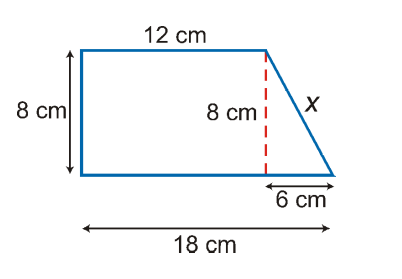
\includegraphics[width=0.3\textwidth]{trapecio}
\end{center}
    
\addpoints

\question[2] Puedes usar los siguientes ejes o dibujar los tuyos propios:\\
    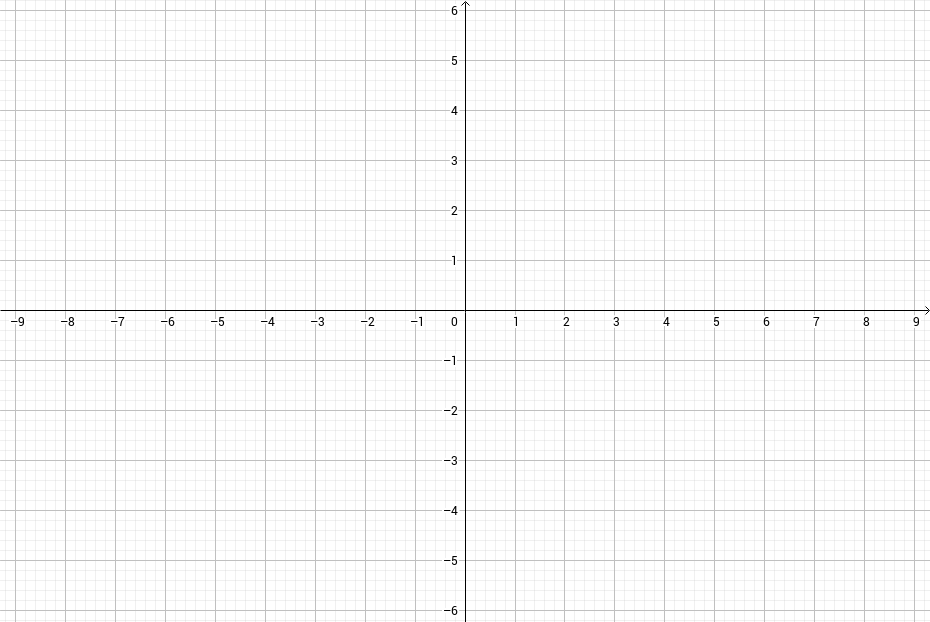
\includegraphics[width=0.9\textwidth]{ejes}

\noaddpoints % to omit double points count
\begin{parts}
\part[1] Representa gráficamente la función $-x+2y=4$
\part[1] Halla la ecuación de la recta que pasa por el punto $P(2,2)$ y cuya pendiente es $-3$. Dibuja la gráfica.
\end{parts}
\addpoints

\question[1] Lanzamos un dado y anotamos la puntuación obtenida. Calcula la probabilidad de obtener:
\noaddpoints % to omit double points count
\begin{parts}
\part[0.5] Un número mayor que $4$.
\part[0.5] Un múltiplo de $3$.
\end{parts}
\addpoints

\question[1]
Explica con tus propias palabras el teorema de Pitágoras. Pon, además, un ejemplo.
\makeemptybox{\fill}


\end{questions}

\end{document}
